\documentclass[a4paper,11pt]{article}

\usepackage{../préambule}

\title{Activité : Aires de rectangles}
\date{}
\author{}

\begin{document}
\maketitle

\begin{greybox}[frametitle={Rappel}]
	L'aire d'un rectangle est donnée par la formule \squared{largeur × hauteur}.
\end{greybox}

\begin{exercice}\ \vspace{0.5em}

	\begin{tikzpicture}[scale=0.2]
		% lignes horizontales
		\draw (0,0) -- (27,0);
		\draw (0,22) -- node[anchor=south]{12cm} (12,22);
		\draw (12,22) -- node[anchor=south]{7cm} (19,22);
		\draw (19,22) -- node[anchor=south]{8cm} (27,22);
		% lignes verticales
		\draw (0,0) -- node[anchor=east]{22cm} (0,22);
		\draw (12,0) -- (12,22);
		\draw (19,0) -- (19,22);
		\draw (27,0) -- (27,22);
	\end{tikzpicture}
	\begin{itemize}
		\item Écrire une expression permettant de calculer la \textit{largeur} de ce rectangle. \vspace{1em}
		\item Écrire une expression permettant de calculer l'aire total du rectangle en un coup, en n'utilisant que les nombres présents sur la figure.
		\item Quelle est l'aire du rectangle ? \vspace{1em}
	\end{itemize}
\end{exercice}

\begin{exercice}\ \vspace{0.5em}

	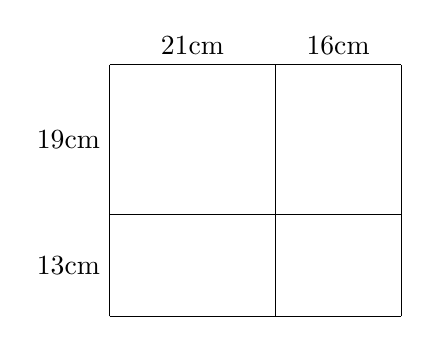
\begin{tikzpicture}[scale=0.1]
		% lignes horizontales
		\draw (0,0) -- (37,0);
		\draw (0,13) -- (37,13);
		\draw (0,32) -- node[anchor=south]{21cm} (21,32);
		\draw (21,32) -- node[anchor=south]{16cm} (37,32);
		% lignes verticales
		\draw (0,0) -- node[anchor=east]{13cm} (0,13);
		\draw (0,13) -- node[anchor=east]{19cm} (0,32);
		\draw (21,0) -- (21,32);
		\draw (37,0) -- (37,32);
	\end{tikzpicture}
	\begin{itemize}
		\item Écrire une expression permettant de calculer la \textit{largeur} de ce rectangle. \vspace{1em}
		\item Écrire une expression permettant de calculer la \textit{hauteur} de ce rectangle. \vspace{1em}
		\item Écrire une expression permettant de calculer l'aire total du rectangle en un coup, en n'utilisant que les nombres présents sur la figure. \vspace{1em}
		\item Quelle est l'aire du rectangle ?
	\end{itemize}
\end{exercice}

\newpage

\begin{exercice*}[Bonus]\ 

	\begin{center}
		\begin{tabular}{ccc}
			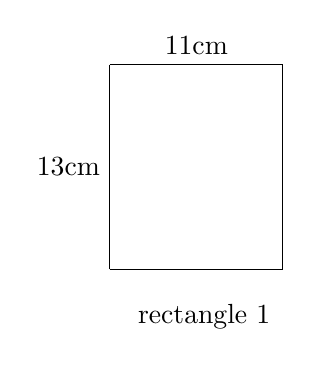
\begin{tikzpicture}[scale=0.2]
				% lignes horizontales
				\draw (0,0) -- (11,0);
				\draw (0,13) -- node[anchor=south]{11cm} (11,13);
				% lignes verticales
				\draw (0,0) -- node[anchor=east]{13cm} (0,13);
				\draw (11,0) -- (11,13);
				% caption
				\node at (6,-3) {rectangle 1};
			\end{tikzpicture} \hspace{4em} &
			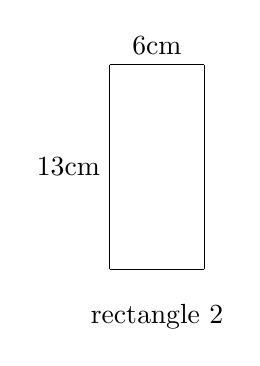
\begin{tikzpicture}[scale=0.2]
				% lignes horizontales
				\draw (0,0) -- (6,0);
				\draw (0,13) -- node[anchor=south]{6cm} (6,13);
				% lignes verticales
				\draw (0,0) -- node[anchor=east]{13cm} (0,13);
				\draw (6,0) -- (6,13);
				% caption
				\node at (3,-3) {rectangle 2};
			\end{tikzpicture}
		\end{tabular}

		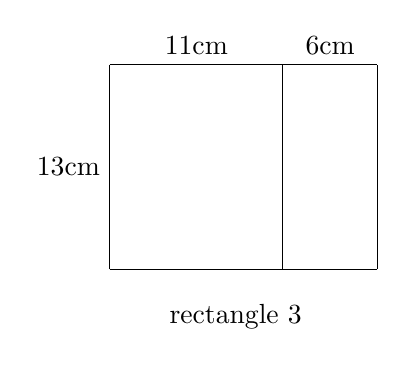
\begin{tikzpicture}[scale=0.2]
			% lignes horizontales
			\draw (0,0) -- (17,0);
			\draw (0,13) -- node[anchor=south]{11cm} (11,13);
			\draw (11,13) -- node[anchor=south]{6cm} (17,13);
			% lignes verticales
			\draw (0,0) -- node[anchor=east]{13cm} (0,13);
			\draw (11,0) -- (11,13);
			\draw (17,0) -- (17,13);
			% caption
			\node at (8,-3) {rectangle 3};
		\end{tikzpicture}
	\end{center}

	\begin{itemize}
		\item Écrit une expression pour calculer l'aire de chacun des rectangles 1 et 2. \vspace{2em}
		\item Écrit une expression pour calculer l'aire du rectangle 3. \vspace{1em}
		\item Écrit une expression qui combine l'aire des rectangles 1 et 2 pour obtenir l'aire du rectangle 3.
	\end{itemize}
\end{exercice*}

\end{document}